% !TEX root = tesis.tex

\chapter{Detección de partículas energéticas\\ solares con el SciCRT}
\chaptermark{Detección de partículas}
\label{chap:cuatro}
\section{Desempeño del SciCRT como detector de RC}

Estudios sobre el desempeño del SciCRT como detector de rayos cósmicos se encuentran en \cite{ynagai14,ysasai14}, sin embargo hacen la evaluación durante un periodo de tiempo corto y condiciones operacionales distintas a las actuales. En la presente sección enfocaré mis esfuerzos en determinar el desempeño del detector bajo las condiciones actuales de operación, con vistas a determinar su confiabilidad durante un evento de partículas solares y estimar los errores sistemáticos.

Con el fin de alcanzar este objetivo utilicé un código de simulación que incluye las descripción completa del telescopio, el cual fue desarrollado por mi colega Rocío García. Los detalles de esta simulación se presentan en \cite{garcia20}. Algunos puntos que fueron necesarios adaptar para mi análisis son los siguientes:

\begin{itemize}
  \item Considerar siete tipos de partículas diferentes: neutrones, protones, $\mu^{\pm}$, $e^{\pm}$ y rayos $\gamma$.
  \item Utilizar el modelo PARMA como generador de eventos para las distribuciones de energía y de ángulos cenitales.
  \item Los parámetros de entrada del modelo son los correspondientes a la localidad de Sierra Negra y el periodo de observación de Septiembre de \num{2017}.
  \item Todas los espectros de energía de las partículas usadas en la simulación se definen en un rango de \SI{10}{\mega\electronvolt} a \SI{1}{\tera\electronvolt}.
  \item Los propiedades ópticas de los materiales del detector están deshabilitadas para reducir el tiempo de computo.
  \item Se simulan en total \num{3e7} de eventos, los cuales son lanzados al detector desde una esfera de \SI{5}{\metre} de radio.
\end{itemize}

La figura \ref{fig:sim-setup} muestra la geometría usada en la simulación para inyectar las partículas al detector. El cubo azul representa la posición del detector en la simulación, mientras que las partículas son inyectas desde la esfera.

\begin{figure}
        \centering
        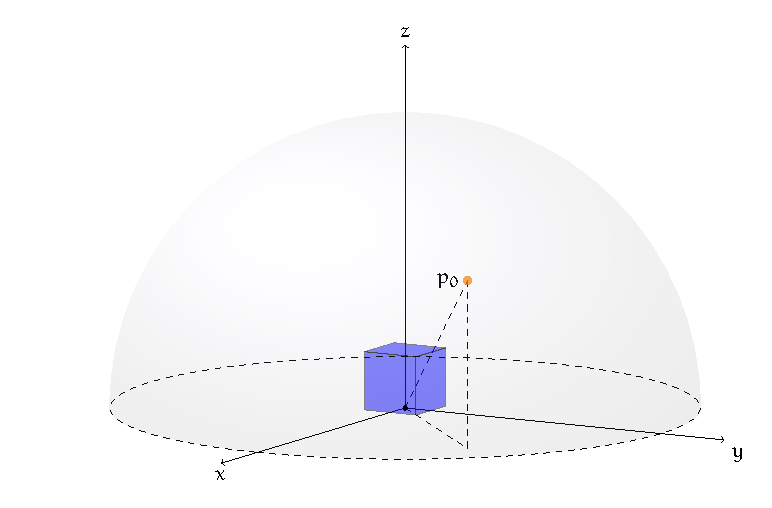
\includegraphics[width=0.75\textwidth]{sim-setup.pdf}
        \caption{Configuración de la simulación en Geant4.}
        \label{fig:sim-setup}
\end{figure}

La condición para que las partículas sean contadas en la simulación es que éstas depositen al menos \SI{7}{\mega\electronvolt} en una barra de cada lado del detector; sin generar señal en las capas dedicadas a la detección de muones. A partir de aquí seleccioné solo los eventos que cumplen con el disparo en el SB \num{3}, que es donde está instalada la electrónica de alta velocidad. El resultado de este análisis se muestra en la figura \ref{fig:total-efficiency}. La línea roja representa la eficiencia de detección de neutrones; mientras que las lineas verde, café, morada, azul y naranja son eficiencias de protones, $\mu^{\pm}$, rayos $\gamma$, positrones y electrones; respectivamente. En todos los casos las eficiencias reportadas son las totales, es decir, están ponderadas con respecto a la distribución angular e incluyen una barra de error. La tasa de eventos total estimada a partir de estas especies es de \SI{3132.31(9480)}{eventos \per\minute}, de los cuales el \SI{84}{\percent} son generados por neutrones.

Las partículas cargadas son rechazadas de manera eficiente usando la señal de anti-coincidencia, sin embargo éstas puede entrar por los lados del detector. Aun así, dado que electrones, positrones y muones depositan en promedio poca energía por barra (aunque tienen una deposición de energía grande en el detector), el umbral de \SI{7}{\mega\electronvolt} constituye una barrera para estas especies. El caso de los protones es más complejo
puesto que pueden tener deposiciones de energía similares a las de los neutrones. De esta forma cerca del \SI{12}{\percent} de los eventos totales son producidos por protones.

De acuerdo con este estudio, el SciCRT tiene una eficiencia de detección grande para rayos $\gamma$ con ángulos mayores a \SI{30}{\degree}; lo cual hace muy limitada su contribución al total de eventos producidos por rayos cósmicos secundarios.

\begin{figure}
        \centering
        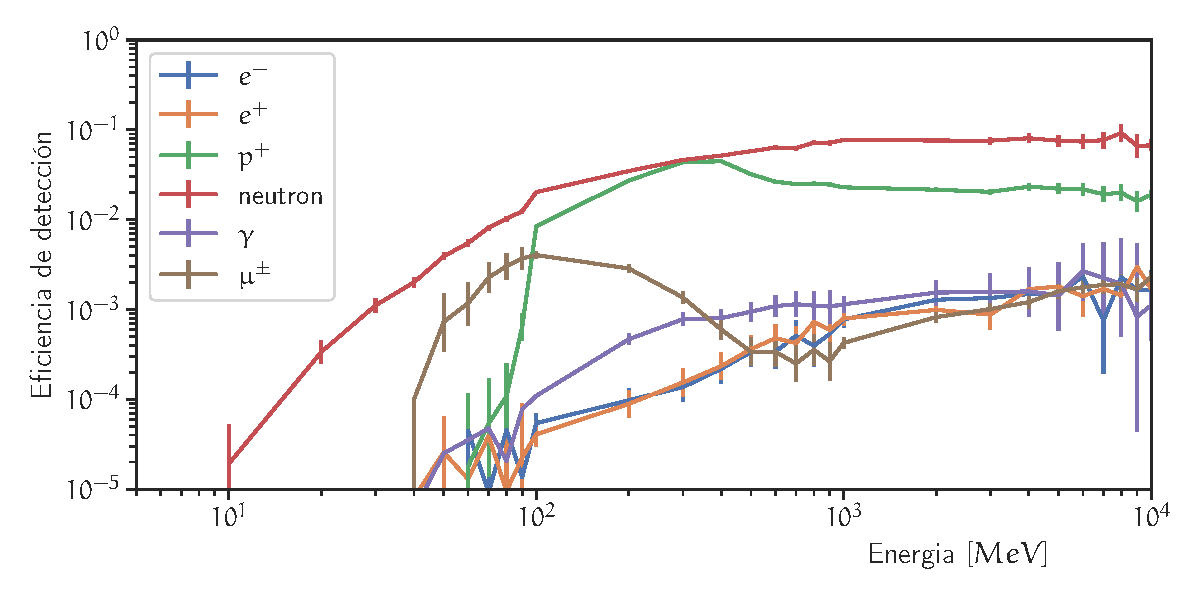
\includegraphics[width=\textwidth]{scibar-efficiency.pdf}
        \caption{Eficiencia de detección del SciCRT para diferentes especies de partículas en función de la energía incidente.}
        \label{fig:total-efficiency}
\end{figure}

El siguiente paso de mi análisis fue comparar la tasa estimada mediante la simulación con los datos experimentales. Los datos usados en este parte del análisis provienen del \num{14} de Noviembre de \num{2017}. La tasa de eventos crudos registrada por el telescopio se muestra en la figura \ref{fig:neutron-1pix}. De este modo la tasa media de eventos se estima en: \SI{3841.68(214)}{eventos \per\minute}.

\begin{figure}
        \centering
        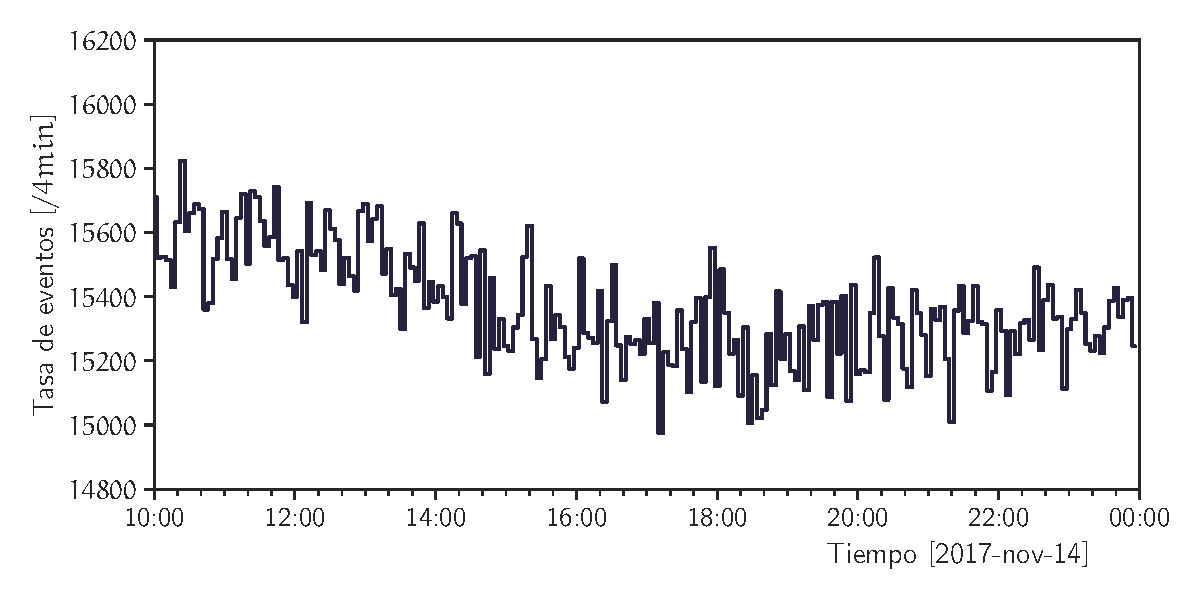
\includegraphics[width=\textwidth]{neutron-171114-1pix.pdf}
        \caption{Tasa de eventos registrada por el SB3 durante el \num{14} de Noviembre de \num{2017}}
        \label{fig:neutron-1pix}
\end{figure}

La diferencia entre la simulación y el experimento es evidente, con un error de \SI{\approx 20}{\percent} tomando como base la simulación. En principio las diferencias deben ser ocasionadas por características del detector no incluidas en la simulación, como pueden ser; las ganancias de los MAPMTs, no linealidades de la electrónica y fluctuaciones debidas a la temperatura, entre otros factores. Dado que las fluctuaciones debidas a la temperatura se deben observar en escalas de tiempo mayores, en primera instancia quedan descartadas como posibles factores que expliquen la discrepancia.

Para poder investigar cualquiera de las posibilidades restantes es necesario reconstruir los eventos registrados por el detector. En resumen este proceso consta de: eliminar el pedestal de las distribuciones de ADC, corregir el efecto de atenuación en las barras y finalmente convertir los valores de ADC en energía depositada.

Una ejemplo de distribución ADC de una de las barras de centelleo se muestra en la figura \ref{fig:neutron-pedestal}. Dos de las características importantes de estas distribuciones son el pico debido a ruido electrónico (pedestal) y el pico de señal (en este caso aproximadamente en \SI{100}{ADC}). Para cada archivo de eventos registrados es necesario estimar el pedestal de cada barra, ya que éste representa el punto de referencia a partir del cual la electrónica mide la energía depositada. La posición del pedestal de cada barra la estimo a partir de la media de una distribución Gaussiana ajustada al pico principal. La distribución que se muestra en la figura \ref{fig:neutron-pedestal} corresponde a los datos de una barra, acumulados durante una día y a los que se les ha sustraído el pedestal.

\begin{figure}
        \centering
        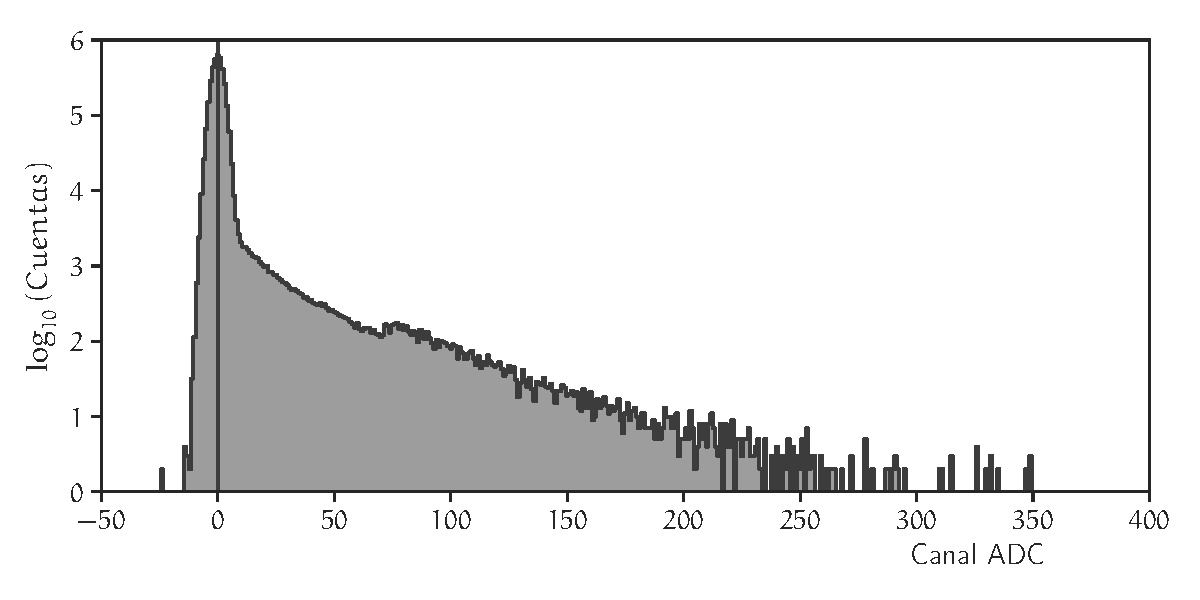
\includegraphics[width=\textwidth]{neutron-ped.pdf}
        \caption{Distribución ADC de una barra de centelleo.}
        \label{fig:neutron-pedestal}
\end{figure}

Posteriormente, es necesario corregir los datos de ADC por efectos de la atenuación en la fibra. Este procedimiento se realiza a través de la ecuación \ref{equ:fiber-att}, mencionada previamente. Finalmente los datos de ADC son convertidos a energía depositada usando el mapa de ganancias descrito en \cite{hikimochi16}.

Usando los datos de deposición de energía construí distribuciones del valor máximo de energía depositado por traza, para el periodo de tiempo analizado. El resultado se muestra en la figura \ref{fig:neutron-mindep}, en donde la distribución azul corresponde a las barras del lado Y del SciCRT y la distribución naranja a las del lado X. Estas distribuciones son útiles ya que permiten estudiar el umbral de detección de las barras, y de esta manera nos permiten observar si las diferencias detectadas provienen de la electrónica y/o los MAPMTs. A partir de la figura podemos corroborar que el umbral de detección de las barras es menor a \SI{7}{\mega\electronvolt}, lo cual explica la mayor tasa de eventos en el experimento.

\begin{figure}
        \centering
        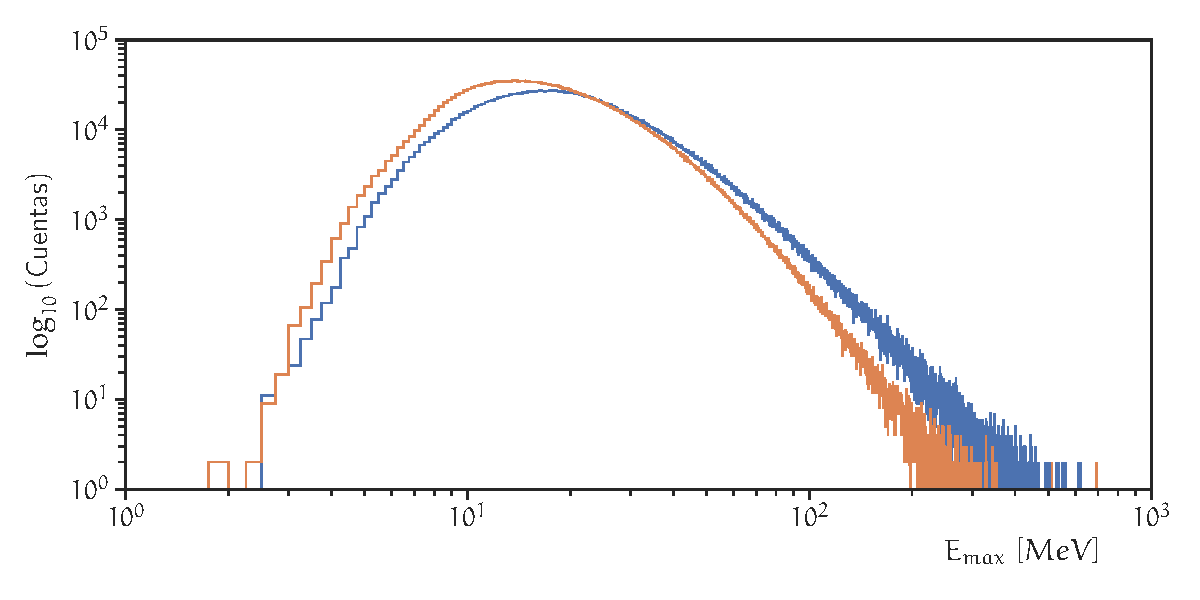
\includegraphics[width=\textwidth]{neutron-mindep.pdf}
        \caption{Distribuciones de energía máxima depositada en una barra de centelleo. La distribución en azul corresponde a las barras del lado Y y la distribución naranja al lado X.}
        \label{fig:neutron-mindep}
\end{figure}

El origen de este fenómeno muy probablemente se debe a unidades de electrónica FE que presentan una ganancia mayor del promedio y por lo tanto amplifican eventos de menor energía. Si bien esta es una deficiencia de la electrónica que afecta la detección de neutrones solares, también es importante remarcar que nos permite registrar una mayor cantidad de eventos de muones y rayos $\gamma$ en el SB3.



\subsection{Estabilidad del detector}

Regarding the stable operation of the SciCRT, Figure \ref{fig:muon-monthly} shows the trigger rate of muon ADC data during February \num{2020} (dark blue line) in comparison with the Neutron monitor (NM) of Mexico City (light blue). The data from the NM has been shifted by \num{1e6} counts to fit the same scale as the SciCRT. As it may be seen from the figure both series follow the same time evolution, despite the fact that the NM is operated under very controlled conditions and the SciCRT is under severe atmospheric conditions at high altitude. To guarantee the operation of the telescope we have installed battery banks and a zero transfer time uninterruptible power supply to prevent the loss data. The DAQ system is also equipped with ai r circulators to enable efficient heat dissipation in the low pressure environment of Sierra Negra.

\begin{figure}
        \centering
        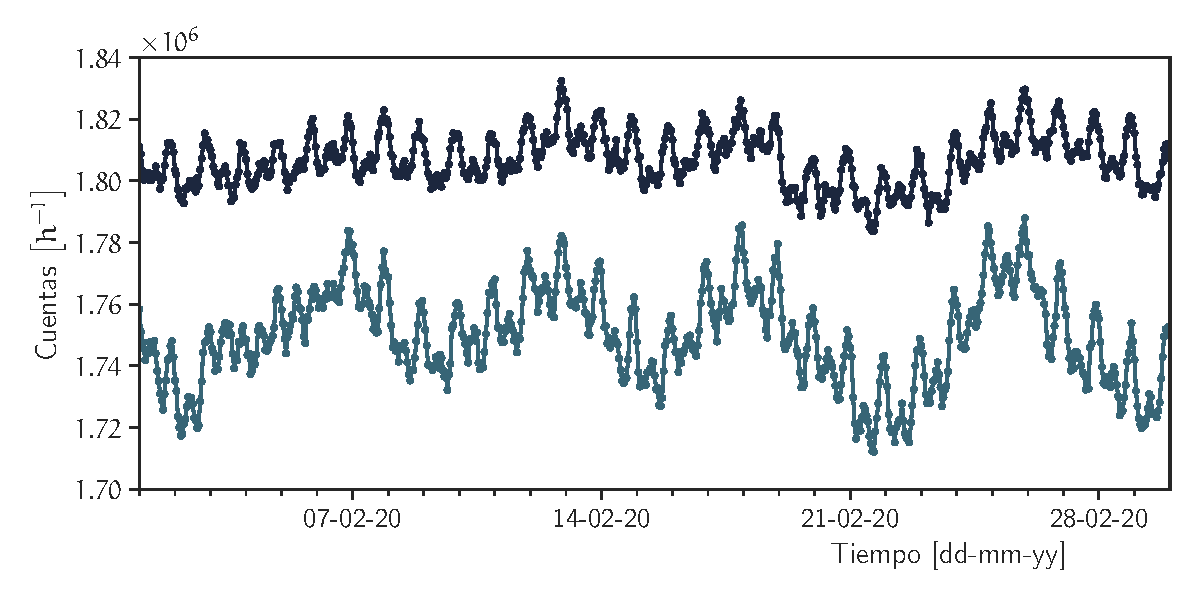
\includegraphics[width=\textwidth]{muon-monthly.pdf}
        \caption{Total de eventos de muones registrados durante Febrero \num{2020} por el SciCRT (linea azul oscura) en comparación con datos del NM de la Ciudad de México (línea azul claro).}
        \label{fig:muon-monthly}
\end{figure}

\begin{figure}
        \centering
        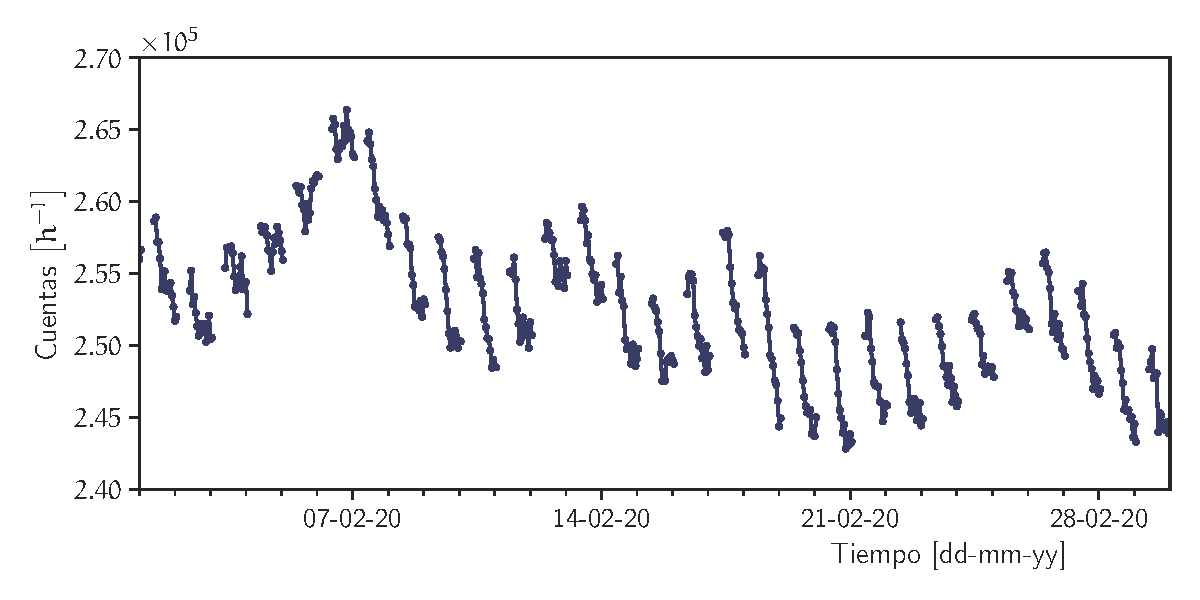
\includegraphics[width=\textwidth]{neutron-monthly.pdf}
        \caption{Total de eventos de partículas neutras registrados durante Febrero \num{2020} por el SciCRT (linea azul oscura) en comparación con datos del NM de la Ciudad de México (línea azul claro).}
        \label{fig:neutron-monthly}
\end{figure}

Figure \ref{fig:mip-stability} shows the gain stability of the MAPMTs used in the neutron layers in the SciCRT. For this analysis we selected a time period of three months, from December \num{2019} to February \num{2020}. The gain is measured determining the peak of the cosmic ray signal in the ADC distribution after pedestal subtraction. The top panel in the figure shows the time variation of one of the MAPMTs from the neutron layers. From this it is clear that the gain of the MAPMT is affected by the conditions at the site, nonetheless all fluctuations laid in the \SI{\pm 2.0}{\percent} interval (light green shaded area) and most of them in the the \SI{\pm 1.0}{\percent} interval (dark green shaded area). The bottom panel in the figure shows the distribution from all the MAPMTs in the neutron layers during the same period of time. Despite the severe atmospheric conditions at Sierra Negra all gain variations are between \SI{\pm 2.5}{\percent}.

\begin{figure}
        \centering
        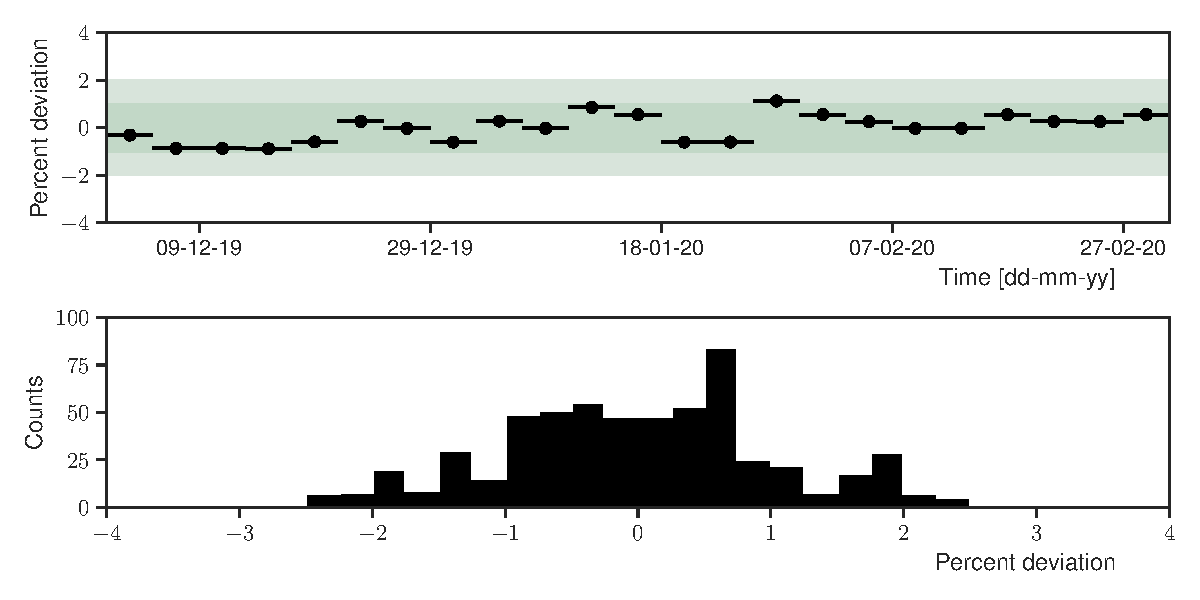
\includegraphics[width=\textwidth]{neutron-mip_stability.pdf}
        \caption{Estabilidad de la ganancia de los MAPMTs durante un periodo de tres meses. El panel superior muestra la variación en el tiempo de uno de los MAPMT. Las áreas sombreadas corresponden con las variaciones de \SI{\pm 1}{\percent} y \SI{\pm 2}{\percent}. El panel inferior es la distribución de todos los MAPMTs.}
        \label{fig:mip-stability}
\end{figure}



\begin{figure}
        \centering
        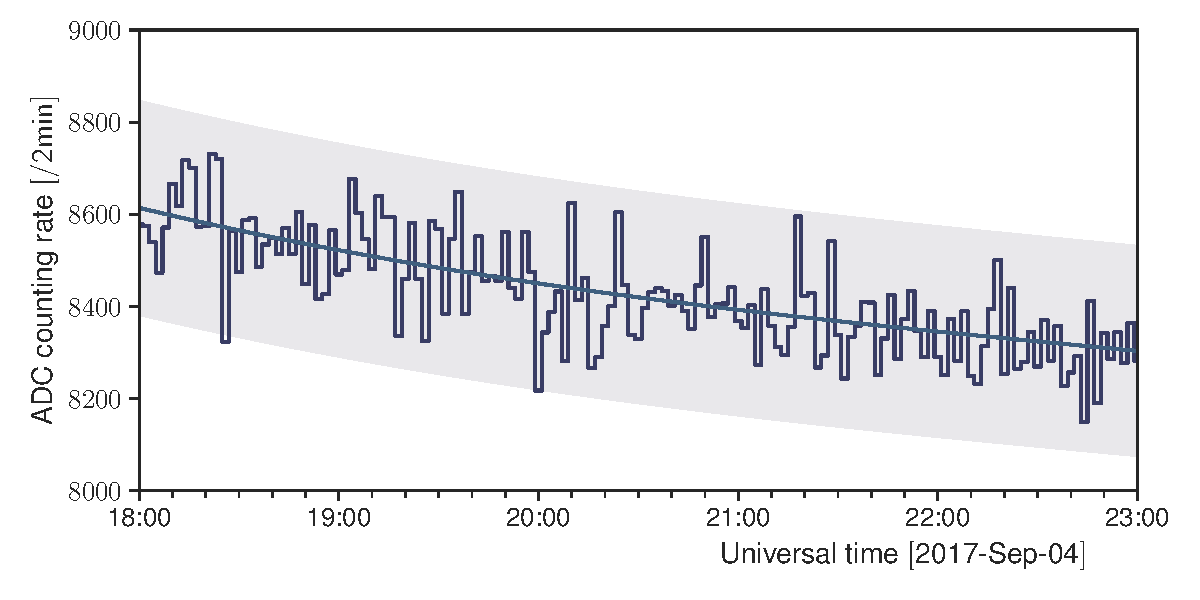
\includegraphics[width=\textwidth]{neutron-170904.pdf}
        \caption{Perfil temporal de eventos registrados por el \emph{SciCRT} el \num{4} de Septiembre de \num{2017}. El área sombreada representa el nivel de $3.0\sigma$.}
        \label{fig:september-04}
\end{figure}

\begin{figure}
        \centering
        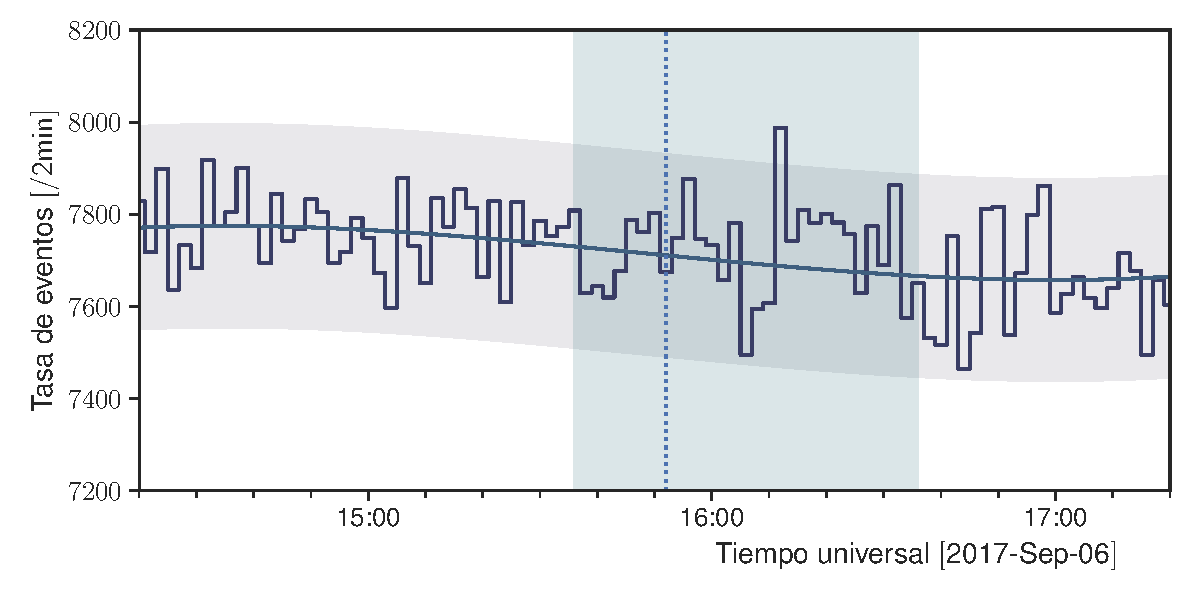
\includegraphics[width=\textwidth]{neutron-170906.pdf}
        \caption{Perfil temporal de eventos registrados por el \emph{SciCRT} el \num{4} de Septiembre de \num{2017}. El área sombreada representa el nivel de $3.0\sigma$..}
        \label{fig:september-06}
\end{figure}
